\chapter{跨域自适应多目标检测与跟踪算法研究}
多目标跟踪系统在真实开放场景(如智能交通、自动驾驶)中的部署,常受雾、低光照等恶劣天气条件的制约。
这些条件导致成像质量退化,形成训练(清晰图像)与测试(恶劣天气图像)之间的输入域差异,
进而造成检测与跟踪性能的显著下降。
尽管第三章提出的跟踪器在清晰域数据上表现出色,
但其性能在跨域场景下仍受限于前端检测模块的退化。

为构建真正鲁棒的跟踪系统,必须在跟踪前端解决输入层面的域自适应问题。
本章针对此问题,提出一套完整的跨域自适应解决方案:
首先,通过可视化分析明确恶劣环境对检测与跟踪的影响(\ref{sec:ch4_1}节);
其次,提出一种基于双渐进滤波的跨域自适应增强器,并与检测器进行端到端协同训练,
实现输入图像的自适应增强(\ref{sec:ch4_2}节);
进而,将训练好的增强-检测模块与冻结的第三章跟踪器集成,
构建完整的“增强-检测-跟踪”推理框架(\ref{sec:ch4_3}节);
最后,通过系统的实验验证所提方法在检测与跟踪任务上的有效性(\ref{sec:ch4_4}节)。
本章工作旨在从源头缓解域偏移,为下游跟踪任务提供鲁棒的视觉表示,是实现跨域自适应跟踪的关键一环。

\section{跨域与恶劣环境问题分析}
\label{sec:ch4_1}
正如本章引言所强调,基于“检测-跟踪”范式的多目标跟踪系统在鲁棒性上表现出显著的强前端依赖性。
尽管后端关联算法(如本文第三章提出的DGCTracker)具备卓越的时空信息建模能力,但其性能上界在本质上仍受限于前端检测器的输出质量。
本节将从数据分布、检测响应、跟踪关联三个层面,逐层分析跨域恶劣环境下的系统退化机理。

\subsection{跨域场景下的数据分布偏移}
现有的主流目标检测器(如 YOLO 系列)大多在COCO\cite{coco}、ImageNet\cite{imagenet}等高质量数据集上进行训练,这些源域数据通常具有直方图均衡、纹理清晰、信噪比高的统计特征。
然而,恶劣天气条件下的目标域数据在像素级统计分布上发生了本质改变:

\begin{itemize}
    \item \textbf{雾天场景(Foggy Domain)}:受大气散射模型影响,图像呈现出非均匀的“白化”干扰。随景深增加,物体表面的对比度呈指数级衰减,高频纹理信息丢失,导致特征提取器难以捕捉清晰的边缘梯度。
    \item \textbf{弱光场景(Low-Light Domain)}:由于成像亮度不足,图像的有效动态范围被压缩至低灰度区间,并伴随明显的色彩失真现象。目标与背景之间的判别性降低,从而削弱了基于外观信息的特征表达能力。
\end{itemize}

上述变化导致目标域数据与源域数据在统计分布上不再满足独立同分布(Independent and Identically Distributed, I.I.D.)假设,使得在源域条件下学习到的卷积滤波器难以在目标域中保持原有的判别能力,从而导致检测与跟踪性能的级联退化。

\subsection{恶劣环境对目标检测性能的影响}
为直观分析恶劣环境对检测性能的影响,本节以 MOT17-02 场景为例,在保持检测模型参数不变的前提下,将原始序列及其弱光、加雾退化版本分别输入 YOLOv3 检测器进行推理,并对检测结果进行定性对比分析。
相关可视化结果如\autoref{fig:ch4_1}所示。
\begin{figure}[htbp]
    \centering
    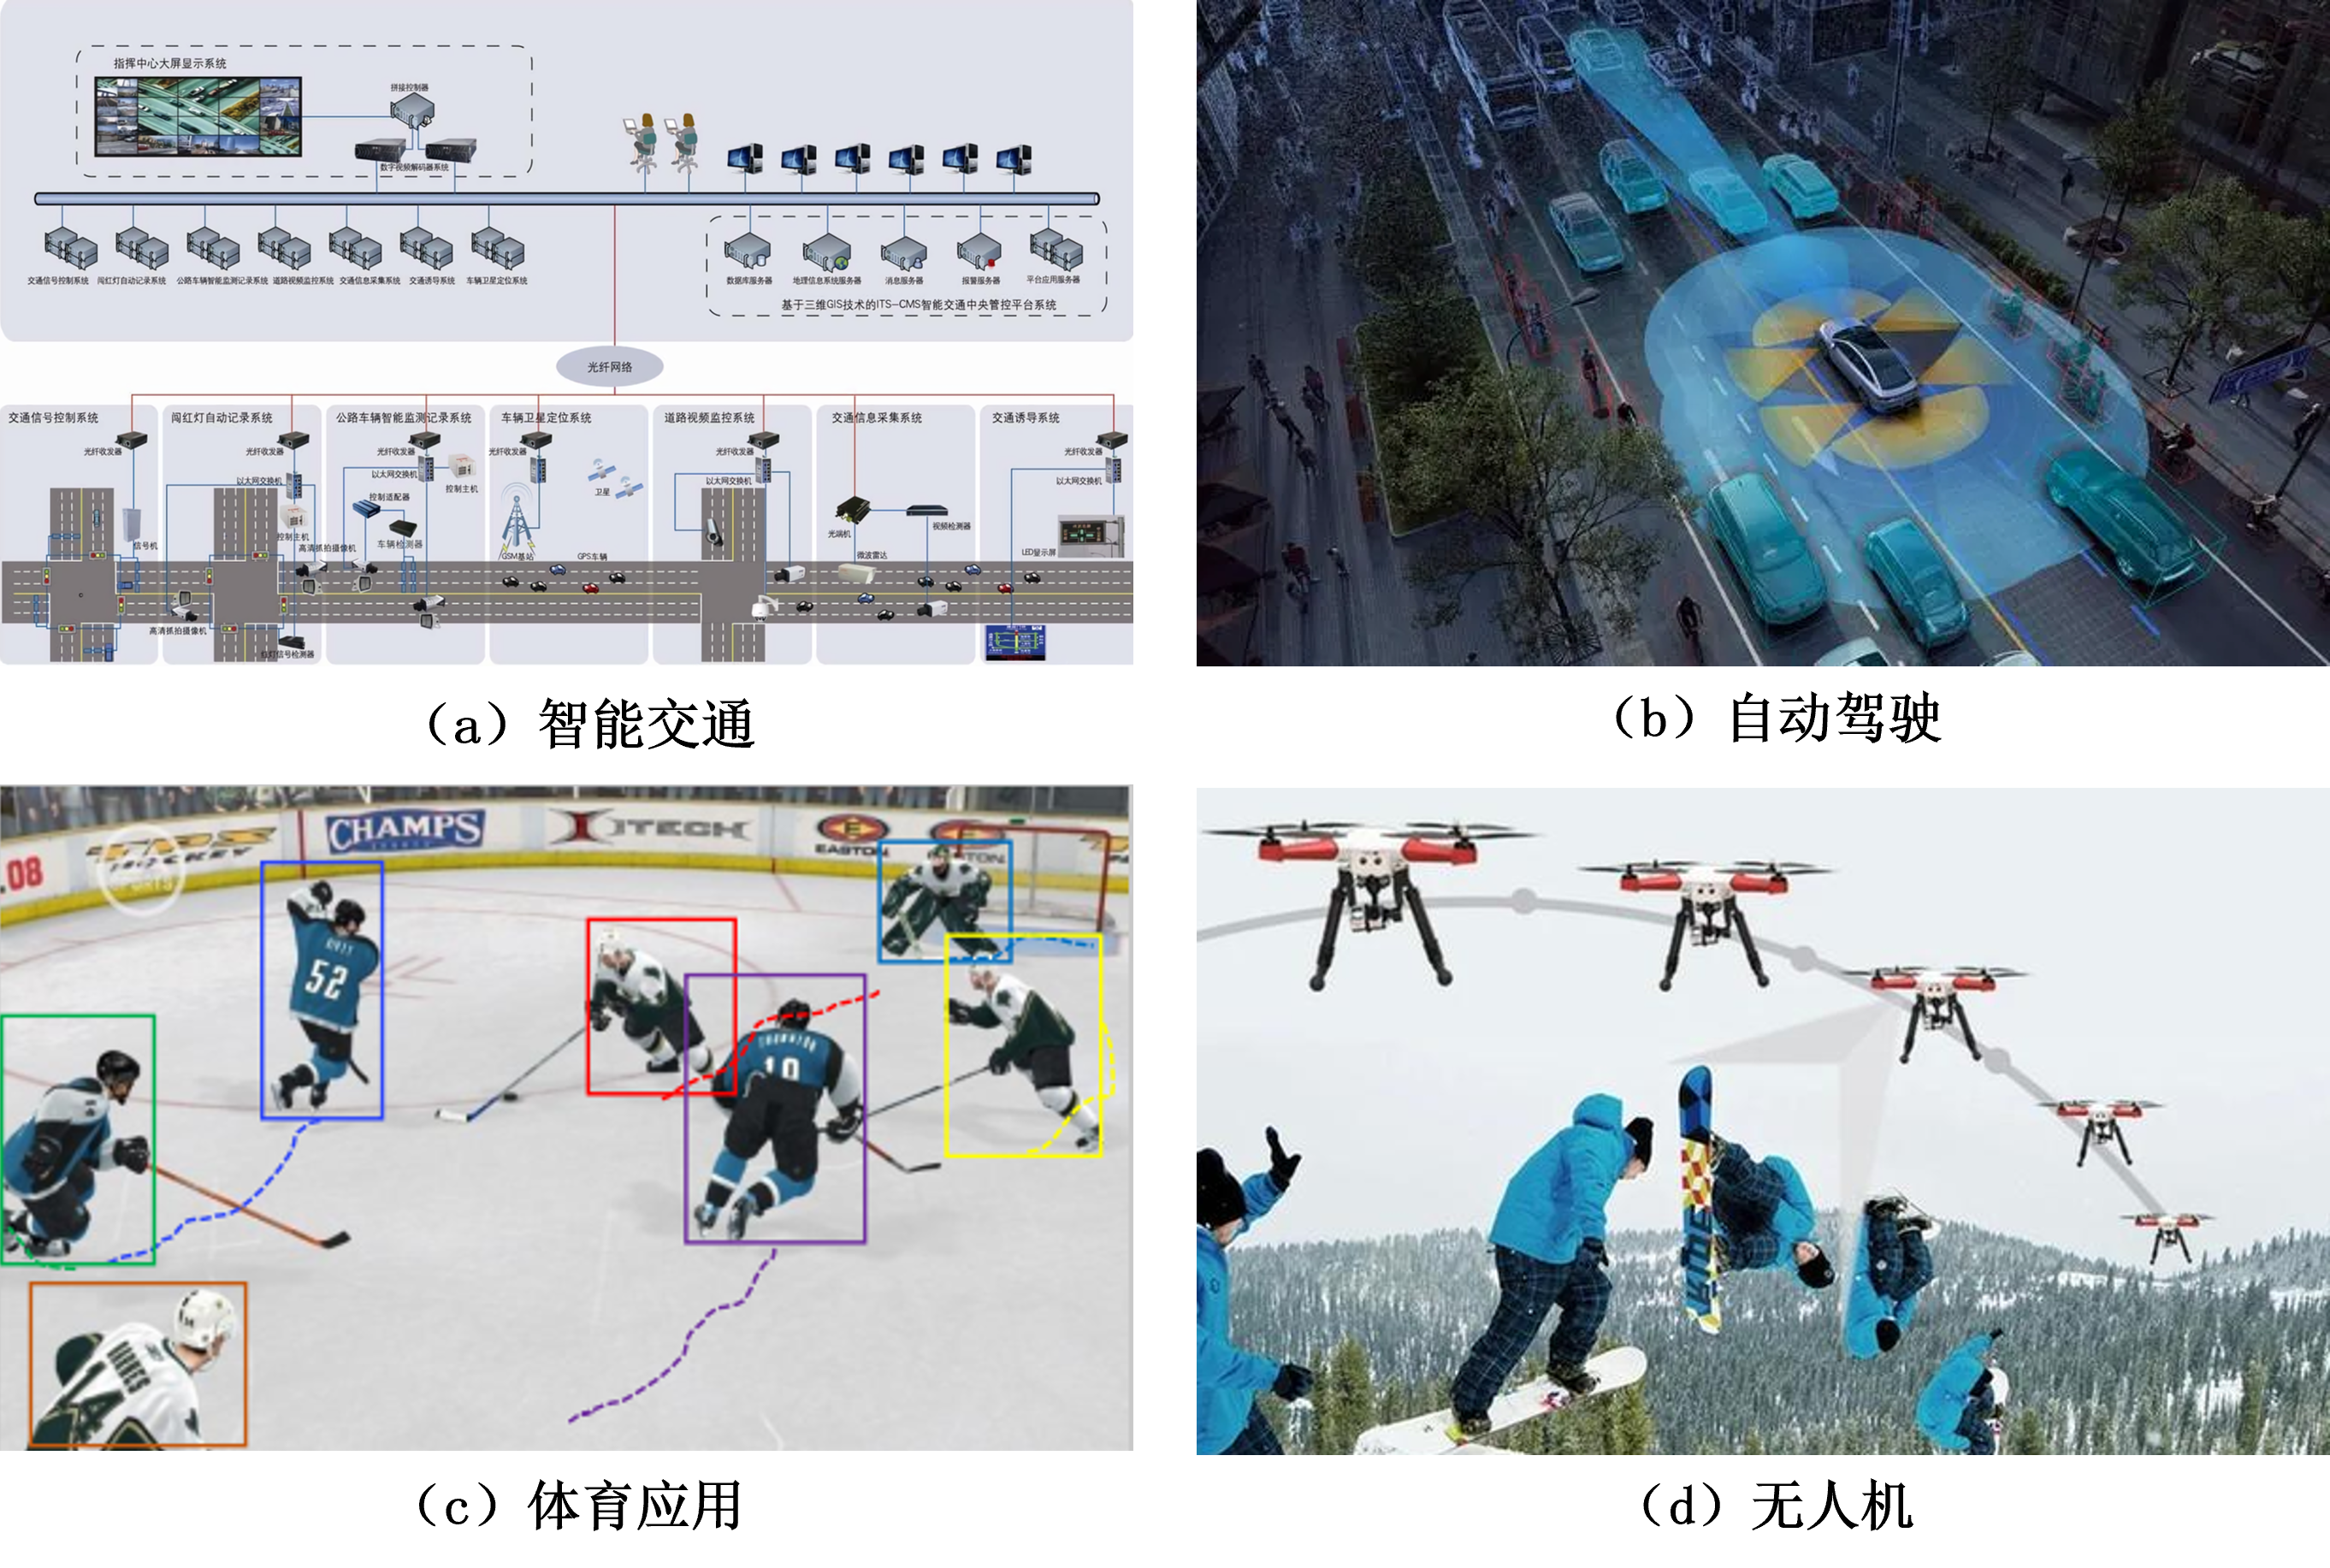
\includegraphics[width=16cm]{chapter4/1.png}
    \caption{\label{fig:ch4_1}跨域场景下检测性能退化的可视化对比}
\end{figure}

从检测结果可以观察到,恶劣环境主要从以下三个方面削弱了目标检测器的输出质量:
\begin{itemize}
    \item \textbf{目标漏检率显著上升}:恶劣环境显著提高了目标的漏检率,尤其是对远距离及小尺度目标影响更为严重。在雾天场景中,大气散射效应削弱了目标的局部对比度,使得目标区域与背景难以区分;而在弱光场景中,成像噪声与亮度压缩共同作用,进一步降低了目标的可检测性。
    \item \textbf{检测置信度降低}:对于未被漏检的目标,其检测置信度虽仍能维持在较高水平,但与清晰场景下普遍高于0.9的置信度相比,存在明确且系统性的下降。这一现象表明,跨域条件下特征表示的稳定性受到影响,使得检测器对目标的分类置信度相对下降。
    \item \textbf{定位精度下降}:由于环境退化模糊了目标的边缘梯度,使得回归网络难以收敛到一致的边界。这种定位精度的丧失,不仅降低了单帧测量的可靠性,也增加了后续基于几何距离进行数据关联的模糊度。
\end{itemize}

综合上述分析可以看出,跨域与恶劣环境条件并非仅导致检测性能指标的数值下降,而是从置信度分布、目标召回以及定位稳定性等多个层面削弱了检测结果作为可靠观测的质量。
这种观测层面的退化将进一步影响依赖检测结果进行状态估计与数据关联的多目标跟踪过程。

\subsection{恶劣环境对多目标跟踪性能的影响}
多目标跟踪(MOT)本质上是一个基于最大后验概率(Maximum A Posteriori Estimation,MAP)的时序推理过程,其核心高度依赖于观测数据的完备性与准确性。
当前端检测器在恶劣环境下输出稀疏(漏检)且含噪(定位漂移)的检测集合时,后端跟踪器的数据关联与轨迹管理等核心机制将发生系统性的失效。如\autoref{fig:ch4_2}所示,这种失效主要表现为两种典型情况:
\begin{figure}[htbp]
    \centering
    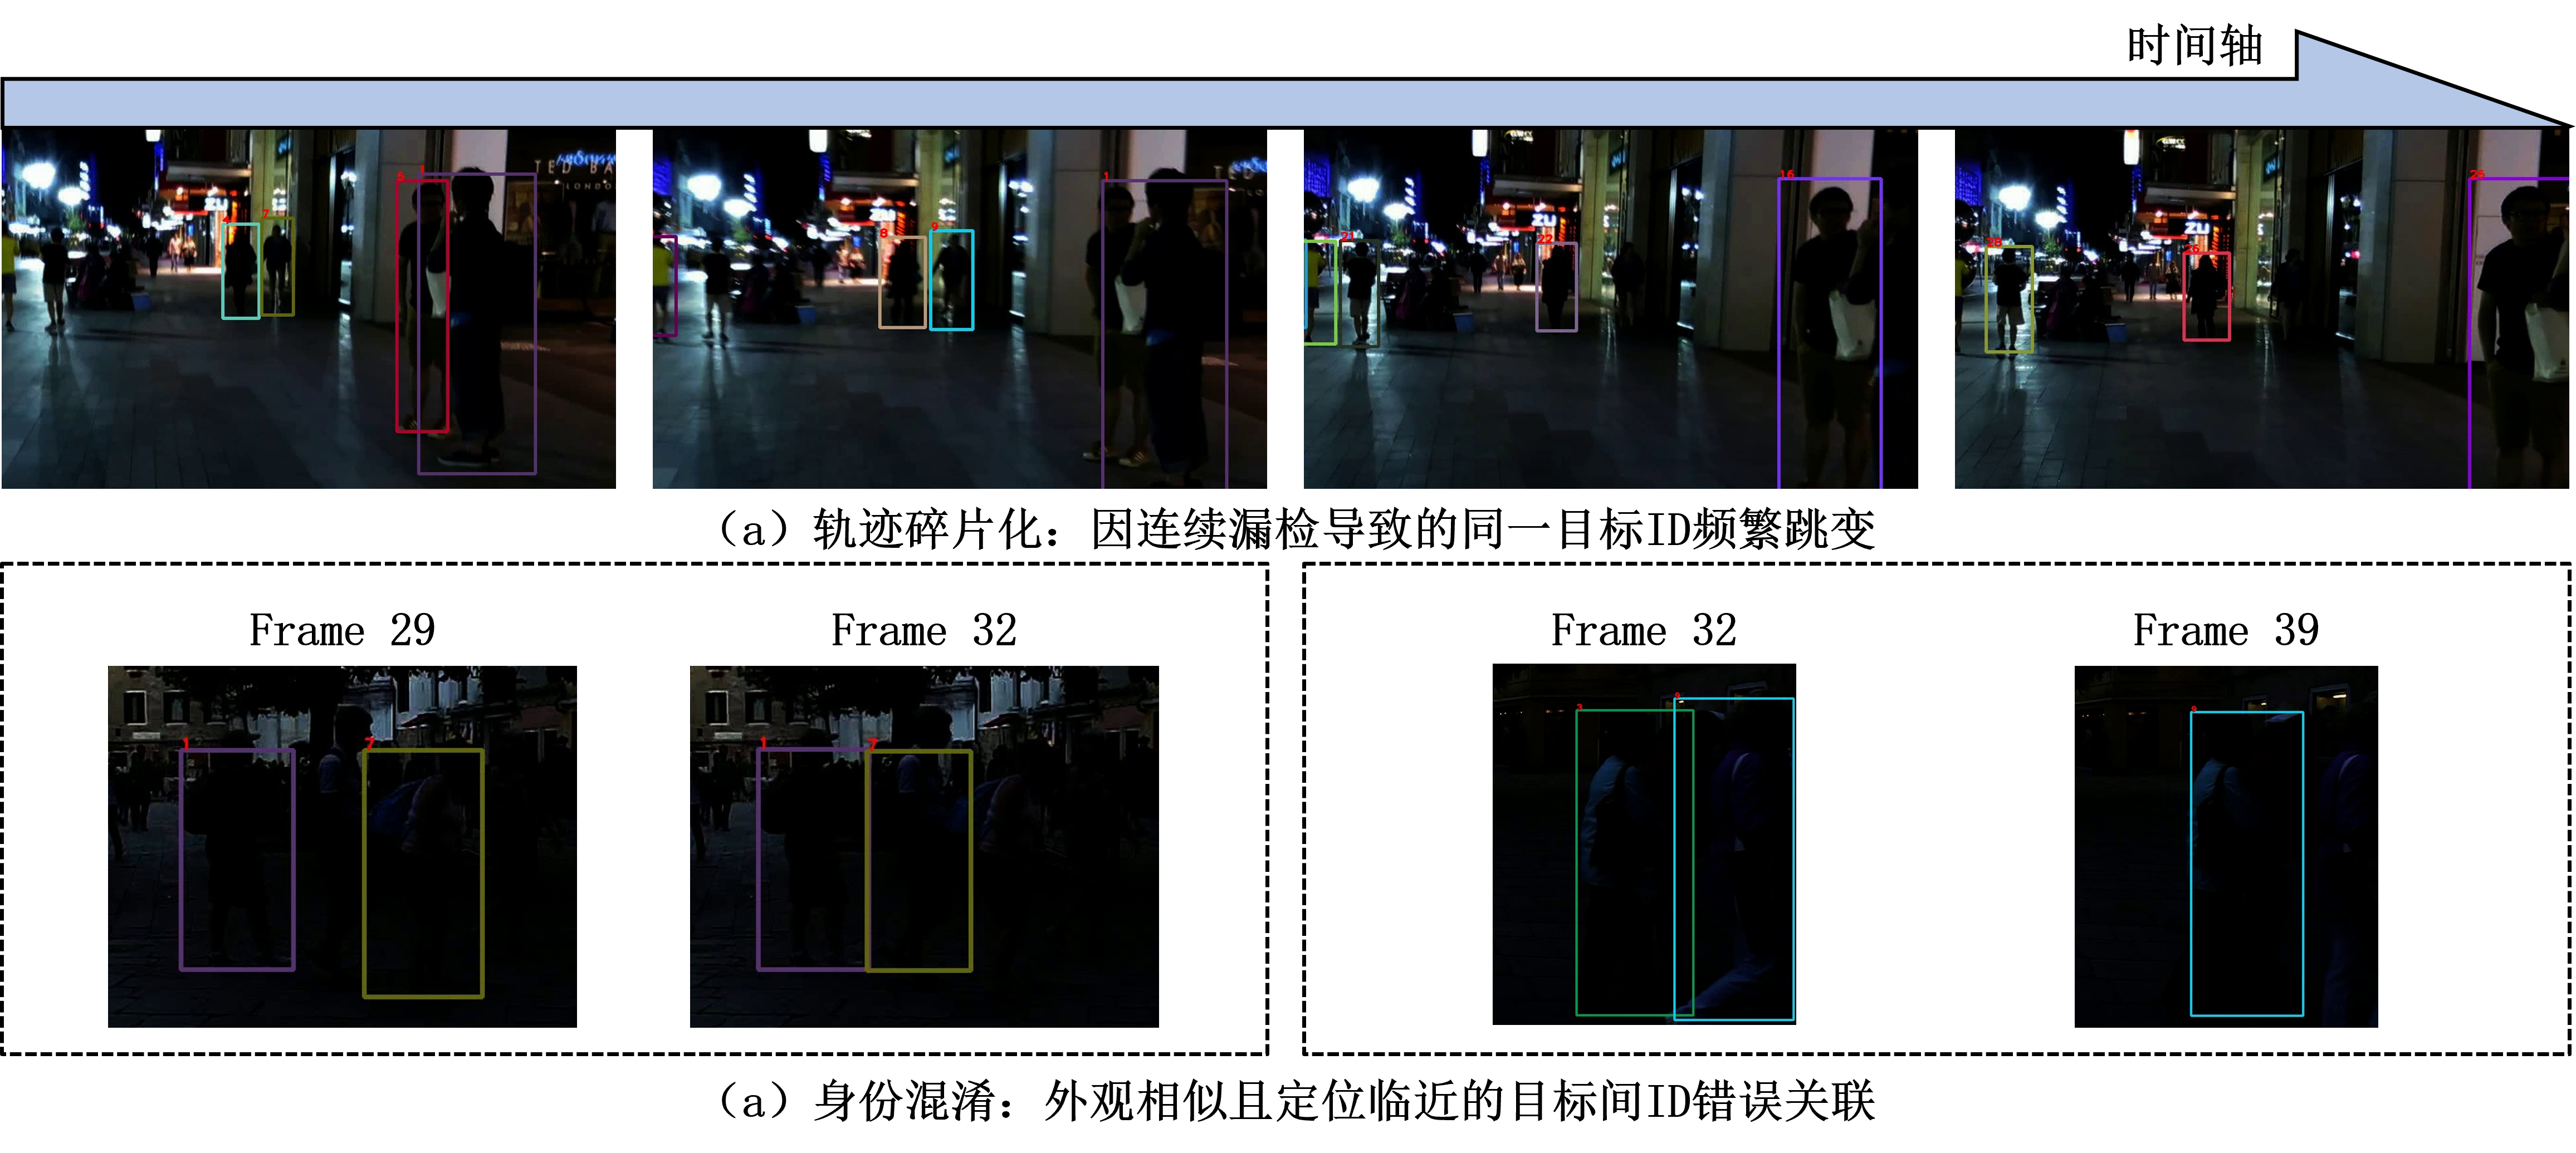
\includegraphics[width=16cm]{chapter4/2.png}
    \caption{\label{fig:ch4_2}弱光环境下多目标跟踪性能退化典型案例}
\end{figure}

\begin{itemize}
    \item \textbf{轨迹碎片化(Trajectory Fragmentation)}:如\autoref{fig:ch4_2}(a)所示,在持续跟踪同一行人的过程中,由于高频的间断性漏检,该目标的检测序列在时间轴上不再连续。这导致跟踪器无法将其关联为一条完整轨迹,而是将其错误地初始化为四条独立的短轨迹(ID=4, 8, 22, 26),造成严重的轨迹碎片化。这种现象使得目标的时序连续性被破坏,大幅增加了轨迹管理的复杂度。
    \item \textbf{身份混淆(Identity Confusion)}:如\autoref{fig:ch4_2}(b)所示,在弱光环境下,空间位置相近且外观相似的多个目标容易发生身份分配错误。该现象主要与恶劣环境下外观特征判别性下降有关。由于成像退化削弱了颜色、纹理等外观线索,由检测框中提取的表观特征在特征空间中的可分性显著降低,使得基于相似度的关联决策变得不稳定,从而增加了身份混淆与错误关联的发生概率。
\end{itemize}

上述两类现象在时间维度上的不断累积,最终表现为多目标跟踪结果整体一致性的显著下降。
轨迹碎片化破坏了目标运动轨迹的完整性,而身份混淆则直接削弱了身份保持能力。
这表明,在跨域与恶劣环境条件下,若不从输入层面改善检测质量与外观表征,仅依赖后端关联算法难以从根本上缓解多目标跟踪性能的退化问题。
因此,本章后续工作将聚焦于设计一个可学习、可集成的前端图像增强模块,旨在直接从输入图像层面补偿域偏移,恢复可靠的观测质量,从而为下游检测与跟踪任务提供保障。
\section{跨域自适应前端增强检测框架}
\label{sec:ch4_2}
针对\autoref{sec:ch4_1}节所揭示的恶劣环境下检测性能退化的问题,本节提出一种前端自适应方案——双渐近滤波增强器(Dual Progressive Filter Enhancer,DPFE),并将其与目标检测器(YOLOv3)进行端到端协同训练,构建
一个统一的跨域自适应增强与检测系统(DPFE-YOLO)。该系统旨在通过可学习的图像增强器,将恶劣天气下的退化图像映射到清晰域,从而恢复检测器所需的高质量视觉特征,从输入层缓解域偏移。
\begin{figure}[htbp]
    \centering
    \includegraphics[width=13cm]{chapter4/3.png}
    \caption{\label{fig:ch4_3}DPFE-YOLO整体框架概览}
\end{figure}

整体框架结构如\autoref{fig:ch4_3}所示,主要由两个核心子系统串联而成:前端的双渐近滤波增强器(DPFE)与后端的目标检测器(如YOLOv3)。
具体而言,原始退化图像首先输入双渐近滤波增强器中。在该模块中,图像先经过视觉编码器提取多层次特征,这些特征随后用于引导一系列级联的双滤波块(Dual Filter Block,DFB)进行渐进式的恢复处理。

为了兼顾全局光照调整与局部去噪的需求,每个DFB内部均采用双路并行的处理架构,包含两个核心可微滤波器与一个门控融合模块:
\begin{itemize}
    \item \textbf{贝塞尔像素级滤波器(Bezier Pixel-wise Filter,BPW)}:该分支利用贝塞尔曲线进行全局像素映射,主要负责图像的亮度增强与对比度拉伸;
    \item \textbf{基于核的局部滤波器(Kernel-based Local Filter,KBL)}:该分支通过动态预测卷积核进行空间滤波,专注于去除雾霾纹理并恢复边缘细节。
\end{itemize}
上述两路滤波分支的输出通过门控机制(Gate)进行自适应加权融合。该机制根据输入特征动态生成权重,决定像素级增强与局部滤波在最终结果中的贡献占比。

最后,经过多级DFB级联增强后的图像被直接送入YOLOv3检测器中,完成目标定位与分类任务。整个系统通过增强损失与检测损失进行端到端联合训练,确保
前端增强器生成的图像特征能最大化地服务于后端的检测性能。

为系统阐述该方法,本节首先介绍所采用的基础可微滤波组件(\ref{subsec:ch4_2_1}节);随后详细阐述
双渐近滤波增强器的结构设计与工作原理(\ref{subsec:ch4_2_2}节);接着说明增强器与检测器协同训练的损失函数与策略(\ref{subsec:ch4_2_3}节);
最后,通过可视化增强器内部状态,展示DPFE的渐进增强与自适应修复机制(\ref{subsec:ch4_2_4}节)。
\subsection{基础滤波组件}
\label{subsec:ch4_2_1}
在双渐近滤波增强器中,图像增强的核心依赖于两个基础滤波组件:贝塞尔像素级滤波器(BPW)和基于核的局部滤波器(KBL)。这两个滤波器均继承自ERUP-YOLO\cite{erup}工作,
分别负责全局像素强度映射与局部空间滤波,共同构成了后续双滤波块(DFB)的核心处理单元。

这种设计是对\ref{subsec:ch2_2_3}节所述的经典可微图像处理方法的进一步升华。现有的 DIP 方法(如 IA-YOLO \cite{ia})通常直接借用传统 ISP 中的固定数学模型(如伽马校正的幂函数、锐化滤波器的线性组合等)。
虽然这些方法具备物理可解释性,但其参数空间往往是不连续的,且单一的物理模型难以拟合复杂多变的恶劣天气退化分布。相比之下,BPW和KBL提供了更具通用性的参数化表达:
BPW是对各类单调色调映射曲线的全局拟合,而KBL则是对各类空间滤波操作的局部统一。本节将详细阐述这两个组件的数学原理和参数化形式。

\textbf{1. 贝塞尔像素级滤波器(BPW)}

BPW滤波器的目标是为图像的每个通道(RGB)学习一个单调递增的非线性映射函数,从而统一实现传统图像处理中的伽马矫正、对比度拉伸和色调映射等全局操作。
该映射通过一个参数化的三次贝塞尔曲线实现。

如\autoref{fig:ch4_4}所示,一条三次贝塞尔曲线由四个控制点定义:起点$P_0=(0,0)$,终点$P_3=(1,1)$,以及两个可学习的控制点$P_1$和$P_2$。
曲线上的点$C(t)=(C_x(t),C_y(t))$由参数$t\in [ 0,1 ]$表示为:
\begin{equation}
    C(t) = (1-t)^3P_0 + 3(1-t)^2tP_1+3(1-t)t^2P_2+t^3P_3
\end{equation}

为保证,映射的单调性及输出范围在$[0,1]$,ERUP-YOLO将控制点$P_1$和$P_2$约束在单位正方形内。
具体地,控制点坐标由可学习参数$r_1$,$\theta_1$,$r_2$,$\theta_2$(每个通道独立)通过下式计算:
\begin{equation}
    \begin{aligned}
        P_1 &= \left(\frac{r_1+1}{2} \cos( \frac{(\theta_1+1)\pi}{4}), \frac{r_1+1}{2}\sin(\frac{(\theta_1+1)\pi}{4})\right) \\
        P_2 &= \left(\frac{r_2+1}{2} \cos( \frac{(\theta_2+1)\pi}{4}), \frac{r_2+1}{2}\sin(\frac{(\theta_2+1)\pi}{4})\right)
    \end{aligned}
\end{equation}
其中,$r_1,r_2\in[-1,1]$,$\theta_1,\theta_2\in[-1,1]$。当所有参数为零时,曲线退化为恒等映射$y=x$。
\begin{figure}[htbp]
    \centering
    \includegraphics[width=13cm]{chapter4/4.png}
    \caption{\label{fig:ch4_4}贝塞尔曲线像素级滤波器(BPW)的映射曲线示例}
\end{figure}

为实现高效的可微运算,ERUP-YOLO采用分段线性近似:将参数区间$t\in[0,1]$均匀划分为$L$段(通常$L=8$),在第$j$段($t\in[t_j,t_{j+1}]$)内,使用线性函数近似曲线,
其斜率为$\Delta C_y(t_j)/\Delta C_x(t_j)$。则对于输入像素强度$p_{in}\in [0,1]$,输出强度$p_{out}$通过下式计算:
\begin{equation}
p_{out} = \sum_{j=0}^{L-1}\text{clip}\left(p_{in} - C_x(t_j),0,\Delta C_x(t_j)\right)\cdot \frac{\Delta C_y(t_j)}{\Delta C_x(t_j)}
\end{equation}
其中,$\text{clip}(x,a,b)$将$x$裁剪到区间$[a,b]$,$\Delta C_x(t_j) = C_x(t_{j+1} - C_x(t_j))$,$\Delta C_y(t_j) = C_y(t_{j+1} - C_y(t_j))$。
该操作对每个RGB通道独立进行,因此BPW滤波器共有$3\times 4=12$个可学习的参数(每通道四个)。

如\autoref{fig:ch4_5}所示,BPW滤波器通过一条可学习的曲线统一个多种全局变换。当曲线呈现上凸形态时,其作用类似于伽马校正($\gamma < 1$)以增强暗部细节;
当下凹时则类似于对比度拉伸;而通过为不同通道学习不同的曲线形状,即可实现自适应白平衡与色调调整。因此,BPW可以视为对\ref{subsec:ch2_2_3}中多个独立像素级滤波器的泛化与统一。
\begin{figure}[htbp]
    \centering
    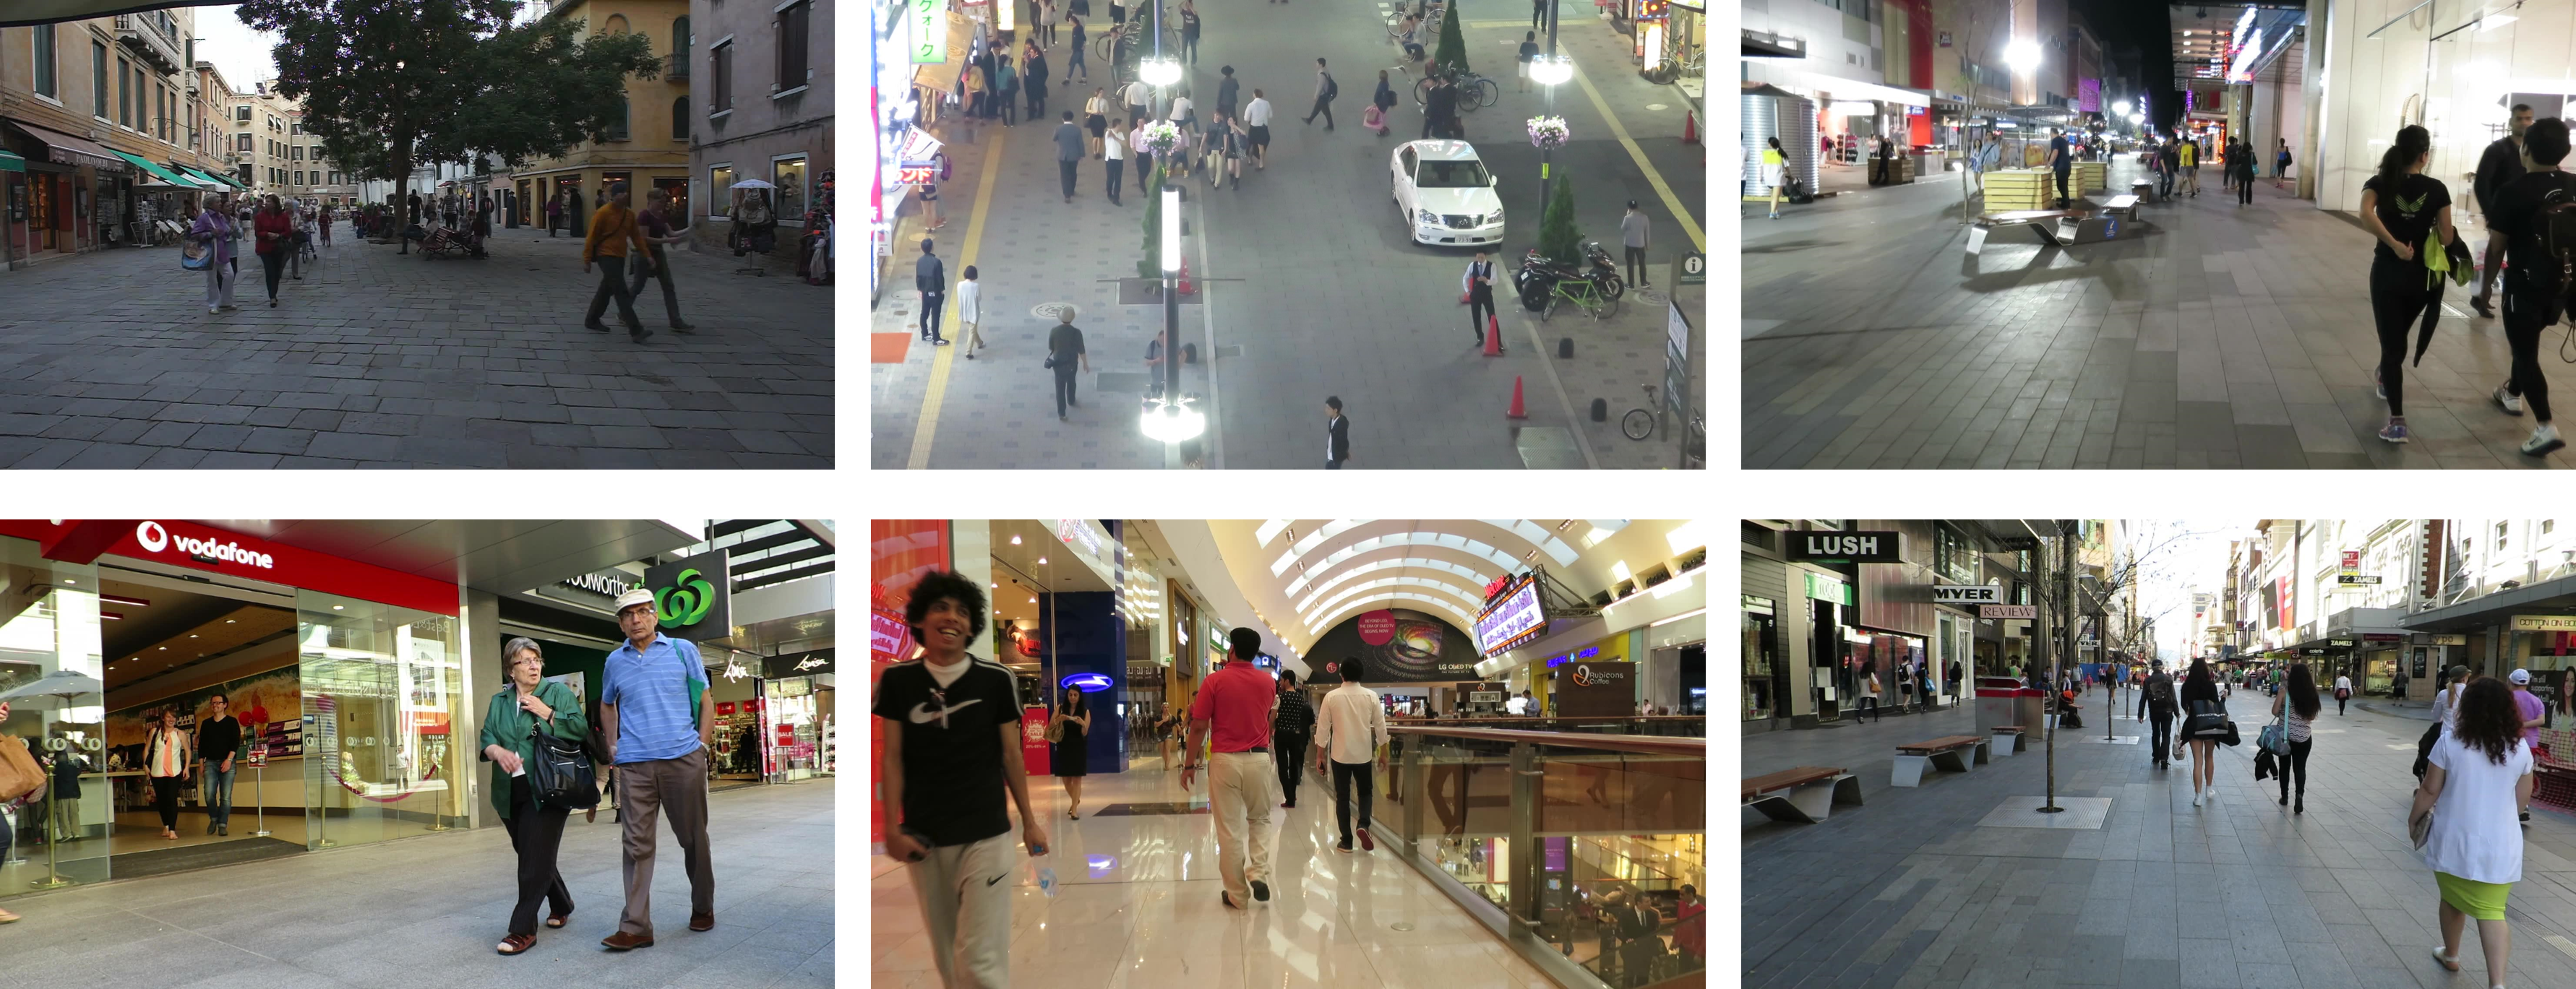
\includegraphics[width=16cm]{chapter4/5.png}
    \caption{\label{fig:ch4_5}贝塞尔曲线像素级滤波器(BPW)与传统像素级滤波器的映射曲线对比(摘自ERUP-YOLO)}
\end{figure}

\textbf{2. 基于核的局部滤波器(KBL)}

KBL滤波器旨在模拟去雾、锐化等依赖于局部邻域的空间滤波操作。其设计灵感来源于传统ISP中的锐化滤波器与基于物理的去雾模型,但将其统一为一种可学习的局部线性卷积形式。

KBL滤波器对输入图像$I$(各通道独立处理)执行如下处理:
\begin{equation}
    F_{KBL}(I) = I \otimes K_1 + I \otimes K_2 + I
\end{equation}
其中$\otimes$表示卷积操作,$K_1$和$K_2$为两个可学习的卷积核(尺寸为$k\times k$,默认设置为$k=9$),分别对应局部调制与细节恢复两项。第一项$I\otimes K_1$可视为对输入图像的局部加权平均,
起到自适应平滑或锐化作用;第二项$I\otimes K_2$则用于添加恢复性的细节成分;最后,一项残差连接保留了原始输入信息,确保梯度顺畅传播。

在ERUP-YOLO中,卷积核$K_1$和$K_2$的参数是由一个小型神经网络从输入图像的特征中动态预测,并通过$\text{tanh}$函数将数值约束在$[-1,1]$区间。然而,这种简单的约束方式
并不能保证卷积核的稳定性,尤其是在训练初期,预测的卷积核可能具有较大的幅值,导致梯度爆炸或训练不稳定。为了增强训练的稳定性和卷积核的可解释性,我们在其基础上提出了一种改进的归一化策略。

具体而言,对于每个通道$c$,预测的核参数首先通过$\text{tanh}$函数约束在$[-1,1]$区间,得到原始卷积核$\tilde{K}_1^c,\tilde{K}_2^c \in \mathbb{R}^{k\times k}$。
然后我们对每个卷积核进行如下归一化操作:
\begin{equation}
    K_i^c = \frac{\tilde{K}_i^c}{ \sum_{u,v}\tilde{K}_1^c(u,v) + \epsilon}, \quad i = 1,2
\end{equation}
其中$\epsilon$为一个小常数(本文取$10^{-8}$),用于防止除零。归一化后的卷积核满足$\sum_{u,v}\tilde{K}_1^c(u,v) \approx 1 $,从而将卷积操作的输出幅值限制在合理范围内。

这种改进的归一化策略具有以下优点:
\begin{enumerate}
    \item \textbf{训练稳定性}:通过约束卷积核的$L1$范数,有效避免了因核权值幅值过大而导致的梯度爆炸或数值溢出,使训练过程更加平稳。
    \item \textbf{可解释性}:归一化后的卷积核可以视为对输入局部区域的加权平均,其权重绝对值之和为1,符合传统空间滤波器的物理含义,便于理解与分析。
    \item \textbf{泛化能力}:归一化操作使滤波器在不同图像和不同退化条件下具有一致的数值尺度,有助于提升模型的泛化性能。
\end{enumerate}

KBL滤波器通过对每个通道使用独立的归一化卷积核,能够灵活地处理不同颜色通道上的退化模式。该滤波器总计有$2\times 3 \times k^2$个可学习参数(两个核、三个通道、每个核$k^2$个参数),
在保持强大表达能力的同时,通过归一化确保了数值稳定性。

KBL滤波器将\ref{subsec:ch2_2_3}节中提到的多种局部滤波操作抽象为一种通用的、数据驱动的局部卷积形式。
其双核设计使得网络能够同时学习平滑噪声与增强细节两种互补操作,从而更灵活地应对雾霾、噪声等多种局部退化。

综上所述,BPW与KBL滤波器分别提供了全局非线性映射与局部空间滤波两种可微的图像处理基元。
它们将传统图像处理操作参数化并嵌入到深度学习框架中,
为后续构建自适应、可学习的增强模块奠定了坚实基础。
与第二章介绍的经典可微滤波器相比,BPW与KBL通过更统一的数学形式和更少的先验假设,
实现了对图像退化更强大的建模能力,是构建下一步图像自适应前端的关键组件。
\subsection{双渐进滤波增强器结构设计}
\label{subsec:ch4_2_2}
基于\ref{subsec:ch4_2_1}节介绍的基础可微滤波组件,本节详细阐述双渐进滤波增强器(DPFE)的整体架构与内部工作机制。
如图\ref{fig:ch4_3}所示,DPFE由视觉编码器(Vision Encoder)与级联的双滤波块(DFB)构成,
其设计遵循“由粗到细”的渐进增强原则,旨在通过多层次的特征引导与自适应滤波,将退化图像逐步恢复至清晰域。以下将依次介绍各核心组件的设计及其协同工作流程。

\textbf{1. 视觉编码器(Vision Encoder)}

视觉编码器作为DPFE的感知前端,负责从输入退化图像中提取多层次特征,
并将每个尺度的特征压缩为固定维度的条件向量,作为对应层次双滤波块(DFB)的条件输入。
我们的视觉编码器设计在ERUP-YOLO的基础上进行了改进,使其特征提取过程更为平滑,以更好地保留空间信息。

编码器的主体由$N$个卷积层(本文取$N=5$)级联构成,每层执行步长为2的卷积操作(使用3×3卷积核),从而实现空间分辨率的逐层减半与通道数的逐层倍增(从64开始,最后一层为1024)。
与ERUP-YOLO中采用的平均池化下采样不同,我们的直接卷积下采样设计减少了信息丢失的风险,并使得特征金字塔的构建更为紧凑。

为进一步缓解早期下采样可能带来的信息损失,我们在编码器前端引入了一个可选的预解码器(Pre-decoder)模块。
该模块由两个步长为2的卷积层组成,将输入图像下采样4倍,同时将通道数逐步提升至32。
这一设计使得从图像空间到特征空间的过渡更加平缓,有利于后续层次的特征学习。

对于每个卷积层输出的特征图,我们通过一个自适应平均池化(Adaptive Average Pooling)层将其空间尺寸压缩至$1\times1$,
随后通过两个$1\times1$卷积层(中间使用SELU激活函数)将通道数调整至统一的编码器输出维度(本文设为256)。
这样,每个层级最终都得到一个256维的特征向量,记为${\mathbf{v}_1, \mathbf{v}_2, \dots, \mathbf{v}_N}$。

相较于ERUP-YOLO中仅使用最后一层特征向量来预测所有滤波器参数的做法,
我们的编码器保留了所有$N$个层级的特征向量,并将其分别输入对应的$N$个DFB块中。
这一设计使得浅层DFB能够利用包含更多细节的低级特征,
而深层DFB则可以利用富含语义信息的高级特征,从而为渐进式增强提供了层次化的条件引导。
\textbf{2. 双滤波块(DFB)}


\textbf{3. 渐进式级联增强}


\subsection{增强-检测端到端协同训练}
\label{subsec:ch4_2_3}
\subsection{自适应增强的可视化分析}
\label{subsec:ch4_2_4}

\section{跨域自适应检测与跟踪推理框架}
\label{sec:ch4_3}

\section{实验结果与讨论}
\label{sec:ch4_4}


\section{本章小结}
\label{sec:ch4_5}
